\section{Wechselstromrechnung}
	\subsection{Allgemein zeitabhängige Grössen}
	\begin{tabular}{|ll|ll|}
    \hline
	\multicolumn{2}{|l}{Arithmetischer Mittelwert, Gleichwert, Linearer MW} 
	    	& \multicolumn{2}{l|}{$X_0 = \overline{X} = X_m = \frac {1} {T} \int\limits_{t_0}^{t_0+T}
	    	x(t)dt$} \\
	\hline
	Quadratischer MW, Leistung 
		& $X^2 = \frac {1} {T} \int\limits_{t_0}^{t_0+T} x^2(t)dt$ 
		& MW $n$. Ordnung
		& $X^n = \frac {1} {T} \int\limits_{t_0}^{t_0+T} x^n(t)dt$ \\
	\hline
	Effektivwert 
		& $X = \sqrt{X^2} = \sqrt{\frac{1}{T} \int\limits ^{t_0+T}_{t_0}{x^2(t)dt}}$
		& Gleichrichtwert 
		& $X_{|m|} = \bar{|X|} = \frac{1}{T} \int\limits_{t_0}^{t_0+T}{|x(t)| dt}$ \\
	\hline
   	\end{tabular}

	\subsection{Begriffe}
		\begin{tabular}{lllll}
		Scheinwiderstand & & $Z = \frac{U_{eff}}{I_{eff}} $ & $ = \sqrt{R^2+X^2}$ &
		Ohm\\ Komplexer Widerstand & Impedanz & $\underline Z = R + jX $ & $ = Z \cdot
		e^{j \varphi}$ & Ohm\\
		Komplexer Leitwert & Admittanz & $\underline Y = G + jB $ & $ =
		\frac{1}{\underline Z} = \frac{1}{Z}e^{-j\varphi}$ & Siemens\\
		Wirkwiderstand & Resistanz & $R = \Real(\underline Z) $ & $ = Z
		\cdot cos(\varphi)$ & Ohm\\
		Wirkleitwert & Konduktanz & $G = \Real(\underline Y) $ & $ \neq \frac{1}{R}$ &
		Siemens\\
		Blindwiderstand & Reaktanz & $X = \Imag(\underline Z) $ & $ = Z
		\cdot sin(\varphi)$ & Ohm\\
		Blindleitwert & Suszeptanz & $B = \Imag( \underline Y) $ & $ \neq \frac{1}{X}$
		& Siemens\\
		Phasenverschiebung & & $\varphi =
		\arctan\left(\frac{\Imag(\underline{Z})}{\Real(\underline{Z})}\right)$ & &
		Radiant\\
		
		\end{tabular}
	
	\subsection{Schaltelemente bei zeitabhängigen Vorgängen}
	\begin{tabular}{p{1.5cm} p{4.3cm} p{1.5cm} p{4.3cm} p{1.5cm} p{4.3cm}}
   		\multicolumn{2}{l}{\textbf{Ohmscher Widerstand R}}
   			& \multicolumn{2}{l}{\textbf{Kapazitität C}}
   			& \multicolumn{2}{l}{\textbf{Induktivität L}} \\
   		\multicolumn{2}{l}{$u$ und $i$ können sprunghaft ändern}
   			& \multicolumn{2}{l}{$u$ kann nicht sprunghaft ändern}
   			& \multicolumn{2}{l}{$i$ kann nicht sprunghaft ändern} \\
   		\parbox{1.5cm}{
			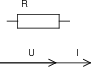
\includegraphics[width=1.5cm]{./bilder/zeigerdiag-r.png}}
			& \parbox{4.3cm}{$u(t) = R i(t)$ \\
				$i(t) = \frac{u(t)}{R}$ \\
				$\underline{Z} = R$}
   			& \parbox{1.5cm}{
				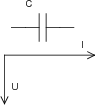
\includegraphics[width=1.5cm]{./bilder/zeigerdiag-c.png}}
			& \parbox{4.3cm}{
				$u(t) = \frac1C \int\limits_0^t i(\tau) d\tau + u(0)$ \\
				$i(t) = C \frac{d u(t)}{dt}$ \\
				$\underline{Z} = \frac{1}{j \omega C} = - \frac{j}{\omega C}$ \\
				$W_C=\frac12 C U_C^2$}
   			& \parbox{1.5cm}{
				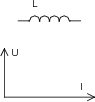
\includegraphics[width=1.5cm]{./bilder/zeigerdiag-l.png}}
			& \parbox{4.3cm}{
				$u(t) = L \frac{di(t)}{dt}$ \\
				$i(t) = \frac1L \int\limits_0^t u(\tau) d\tau + i(0)$ \\
				$\underline{Z} = j \omega L$ \\
				$W_L=\frac12 L I_L^2$}
   	\end{tabular}

	\subsection{Vorgehen bei Schaltvorgängen}
	\fbox{$u(t) =U_E + (U_A - U_E) e^{\frac{-t}{\tau}} \qquad \tau = C R \text{ bzw. }
	\tau =
	 \frac{L}{R} = \frac{\varepsilon}{\sigma} \qquad U_A = \lim\limits_{t
	 \rightarrow 0^+} u(t) \qquad U_E =
	 \lim\limits_{t \rightarrow \infty} u(t)$} $\qquad$ Für Ströme äquivalent
	
	\subsection{Komplexe Darstellung sinusförmiger Vorgänge}
	Momentanwert in $\mathbb{R}$: \fbox{$a(t) = \hat{A} \cos(\omega t + \varphi)$} \qquad
	Momentanwert in $\mathbb{C}$: \fbox{$\underline{a}(t) = \hat{A} e^{j \varphi} e^{j
	\omega t}$} $\qquad$ 
	Amplitude in $\mathbb{C}$: \fbox{$\underline{\hat{A}} = \hat{A} e^{j \varphi}$}\\
	
	Differentiation: $\frac{d}{dt} a(t) = j \omega \underline{\hat{A}}$ $\qquad$ 
	Integration: $\int a(t) dt = \frac{\hat{A}}{j \omega}$
	
	\subsection{Leistungen und Energie}
		\subsubsection{Übersicht}
			\begin{centering}
			\begin{tabular}{|l|c|c|c|c|}
				\hline
					Last & $P=S\cdot\cos\varphi$ & $Q=S\cdot\sin\varphi$ & $S$ & $\cos\varphi$
					\\
				\hline
					rein induktiv & 0 & positiv & $Q$ & 0\\
				\hline
					ohmisch-induktiv & positiv & positiv & $\sqrt{P^2+Q^2}$& $0\cdots1$\\
				\hline
					rein ohmsch & positiv & 0 & $P$ & 1 \\
				\hline
					ohmsch-kapazitiv & positiv & negativ & $\sqrt{P^2+Q^2}$& $0\cdots1$\\
				\hline
					rein kapazitiv & 0 & negativ & $Q$ & 0 \\
				\hline
			\end{tabular}\\
				\end{centering}
		\begin{multicols}{2}
				$S=\sqrt{P^2+Q^2}$\\
				$P=S\cdot \cos \varphi$\\
				$Q=S\cdot\sin\varphi$\\
				$Q=P\cdot\tan\varphi$\\
				$P=Q\cot\varphi$\\
				$\tan\varphi=\frac{Q}{P}$	
		\end{multicols}
	\begin{centering}
	\begin{tabular}{|l|c|c|}
		\hline
			& Parallel-Ersatzschaltung & Reihen-Ersatzschaltung \\
		\hline
			Schaltbild & 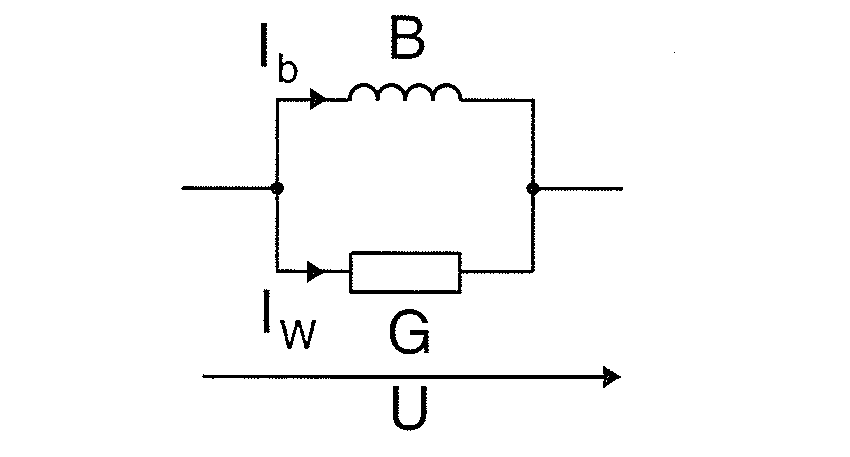
\includegraphics[width=5.5cm]{./bilder/RL_parallel.png} &
			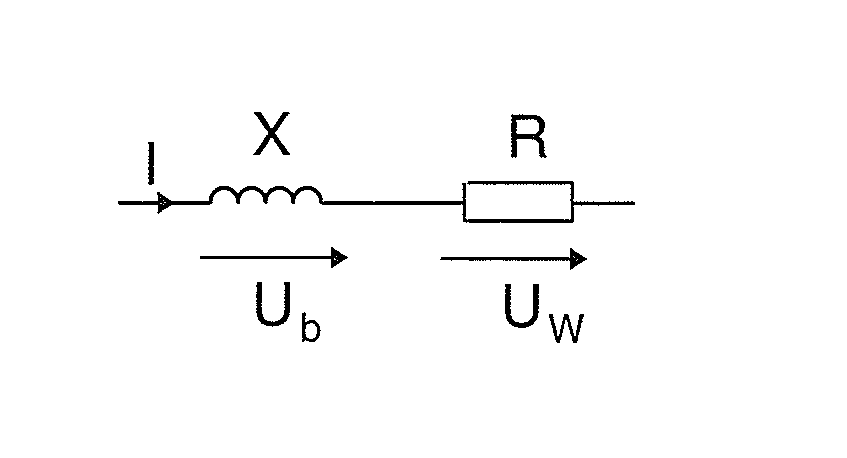
\includegraphics[width=5.5cm]{./bilder/RL_Seriel.png}\\
		\hline
			komplexer Widerstand & & $\underline{Z}=R+jX$\\
			komplexer Leitwert & $\underline{Q}=G+jB$ &\\
		\hline
			Scheinwiderstand & & $Z=sqrt{R^2+X'2}$\\
			Scheinleitwert & $Y=sqrt{G^2+B^2}$ & \\
		\hline
			Wirkwiderstand & & $R=Z\cos\varphi=\frac{U_W}{I}$\\
			Wirkleitwert & $G=Y\cos\varphi_Y=\frac{I_W}{U}$&\\
		\hline
			Blindwiderstand & & $X=Z\sin\varphi=\frac{U_b}{I}$\\
			Blindlietwert & $B = -Z\sin\varphi_Y = \frac{B_b}{U}$&\\
		\hline
			komplexe Leistung & $\underline{Q}=
			\underline{Y^*}U^2=\left(G-jB\right)U^2$& $\underline{S}=\underline{Z}I^2=\left(R+jX\right)I^2$\\
			Wirkleistung & $P=\frac{I_WU=I{_W}{^W}}{G}=U^2G$ &
			$P=U_WI=\frac{U{_W}{^2}}{R}=I^2R$ \\
			Bildleistung & $Q=-I_bU=\frac{-I{_b}{2}}{B}=-U^2B$ & $Q = U_bI =
			\frac{U{_b}{^2}}{X}=I^2X$\\
			Scheinleistung & $S=UI=U\sqrt{I{_W}{^2}+I{_b}{^2}}$ & $S=UI =
			I\sqrt{U{_w}{^2}+U{_b}{^2}}$\\
		\hline
			Wirkfraktor & $\cos\varphi= \frac{G}{Y}$ & $\cos\varphi=\frac{R}{Z}$\\
			Blindfaktor & $\sin\varphi= \frac{B}{Y}$ & $\sin\varphi=\frac{X}{Z}$\\
		\hline
			Wirkstrom & $I_W=I\cos\varphi_Y=GU$ & \\
			Wirkspannung & & $U_W = U\cos\varphi =R \cdot I$ \\
		\hline
			Blindstrom & $I_b = -I \sin\varphi_y = -BU$ & \\
			Blindspannung & & $U_b=U\sin\varphi=X\cdot I$\\
		\hline
	\end{tabular}\\
	\end{centering}
	\begin{tabular}{ll}
   		\parbox{4cm}{
   			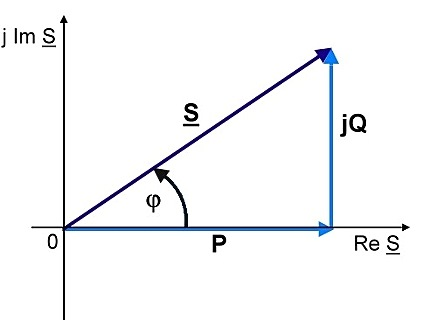
\includegraphics[width=4cm]{./bilder/zeigerdiag-leistungen.png}}
   		& \parbox{14cm}{
			\begin{tabular}{p{3cm}p{5cm}p{5.5cm}}
	      		Momentanleistung
	      			& $p(t) = u(t) i(t)$
	      			\\
				Komplexe Leistung 
					& $ \underline{S} = \underline{U} \cdot \underline{I}^\ast = U\cdot I \cdot
					e^{j(\varphi_u-\varphi_i)}$  & Konjugiert Komplexer Strom! \\
				Wirkleistung
					& $ P = \Real(\underline{S}) = U I \cos(\varphi) $ \\
				Blindleistung 
					& $ Q = \Imag(\underline{S}) = U I \sin(\varphi) $
					& Kapazitiv: $Q < 0$; induktiv: $Q > 0$ \\
				Scheinleistung
					& $ S = | \underline{S} | = U I = \frac{U^2}{R} = I^2 R$ 
					& C: $Q_c=-\omega CU_C^2$, L: $Q_L=\omega LI_L^2$\\
				Leistungsfaktor
					& $\cos \varphi = \frac{P}{S} = \frac{P}{UI}$ \\
				Leistungsanpassung
					& $\underline{Z}_L = \underline{Z}_i^{\ast}; \; P_{max} = \frac{U_q^2}{4
					R_i} = \frac{I_q^2 R_i}{4} $
			\end{tabular}}
   	\end{tabular}

\subsubsection{Blindleistungskompensation}
\begin{tabular}{p{4cm}p{4cm}p{4cm}p{6cm}}
\begin{minipage}{4cm}
    	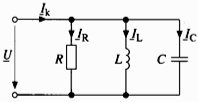
\includegraphics[width=3.5cm]{./bilder/Parallelkompensation.png}
    	\end{minipage}
	& \begin{minipage}{4cm}
    	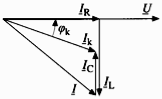
\includegraphics[width=3.5cm]{./bilder/Blindstromkompensation.png}
    	\end{minipage}
	& \begin{minipage}{4cm}
    	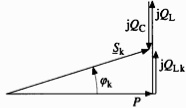
\includegraphics[width=3.5cm]{./bilder/Blindleistungskompensation.png}
    	\end{minipage} 
	& \begin{minipage}{6cm}      
		$$Q_{Lk} = P \cdot \tan{\varphi_k}$$
		$$Q_C = Q_{Lk} - Q_L$$
		$$C = -\frac{Q_C}{\omega U^2}$$
		\end{minipage}
\end{tabular}

\subsection{Systematische Netzwerkanalyse}

\subsubsection{Netzwerkgleichungen, Integro-Differentialgleichungen}
Anstelle der Matrizendarstellung werden hier die Netzwerkgleichungen
vollständig ausgeschrieben mit $\int f(t) dt$ und $\frac{d}{dt} f(t)$.	\\ \\

%\subsubsection{Zweigstrommethode / Kreisstrommethode / Maschenstrommethode}
\begin{tabular}{p{9cm}|p{9cm}}
	\begin{minipage}{9cm}
		%\textbf{Zweigstrommethode}\\
		\subsubsection{Zweigstrommethode}		
		\begin{list}{$\bullet$}{\setlength{\itemsep}{0cm} \setlength{\parsep}{0cm} \setlength{\topsep}{0cm}} 
		\item Maschengleichungen enthalten \textbf{Zweigströme} \\
		$\quad\Rightarrow$ Maschen- \& Stromknotengleichungen benötigt\\
		\item kann nicht in Matrizenform dargestellt werden\\  
        \end{list} 
		\hrule
		\vspace{0.2cm}
		%\textbf{Kreis- oder Maschenstrommethode} (s. Bilder rechts)\\
		\subsubsection{Kreis- oder Maschenstrommethode} (s. Bilder rechts)\\
		\begin{list}{$\bullet$}{\setlength{\itemsep}{0cm} \setlength{\parsep}{0cm} \setlength{\topsep}{0cm}} 
			\item Maschengleichungen enthalten \textbf{Maschenströme}\\
			$\quad\Rightarrow$ nur Maschengleichungen benötigt\\
			\item Kann in Matrizenform dargestellt werden\\
		    \item \textcolor{brown}{Baum} verbindet alle \textcolor{red}{Knoten}, ist
		    aber nie geschlossen\\
		    \item Aufzustellende \textcolor{green}{Maschen} bestehen immer aus beliebig
		    vielen \textcolor{brown}{Ästen} (Zweige vom Baum) und \textbf{einer Sehne}
	    \end{list}	
    \end{minipage} &
	\begin{minipage}{9cm}
    		\underline{Bild 1}\\
    		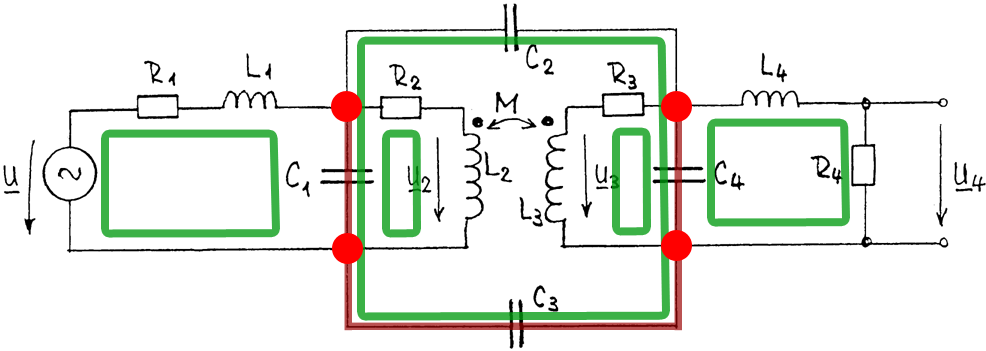
\includegraphics[height=3cm]{./bilder/netzwerkanalyse-kreisstrom2.png}\\
			\underline{Bild 2}\\
			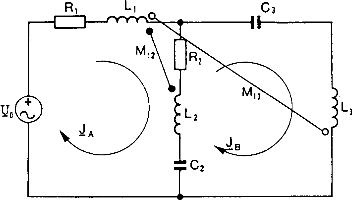
\includegraphics[height=3.5cm]{./bilder/netzwerkanalyse-maschenstrom.png}\\
    		\\
    		\\
    		\hrule
    \end{minipage}\\
\end{tabular} \\
\\ \\
\textbf{Matrix der Maschenstrommethode (Bild 2)}
$$\left[ \begin{array}{cc}
        R_1+R_2 +j \omega L_1 + \frac{1}{j \omega C_2} + j \omega L_2 - j 2
        \omega M_{12} 
    & -(R_2 + j \omega L_2 + \frac{1}{j \omega C_2} - j \omega M_{12} -
        j \omega M_{13}) \\
    -(R_2 + j \omega L_2 + \frac{1}{j \omega C_2} - j \omega M_{12} - j
        \omega M_{13})
    & R_2 + j \omega L_2 + j \omega L_3 + \frac{1}{j \omega C_2} +
        \frac{1}{j \omega C_3}
\end{array}\right] \cdot
\left[ \begin{array}{cc}
     \underline{J}_A \\ \underline{J}_B
     \end{array}\right] =
\left[ \begin{array}{cc}
     U_0 \\ 0
     \end{array}\right]$$
$$\textbf{Allgemein: }\left[ \begin{array}{cc}
       \text{Impedanzen $\underline{Z}$} \\
       \text{symmetrisch zur Diagonalen}
%       \text{Diagonale positiv, sonst negativ}
       \end{array}\right] \cdot \left[ \begin{array}{cc}
     \text{Maschenströme $\underline{J}$}
     \end{array}\right] =
\left[ \begin{array}{cc}
     \text{Spannungsquellen $\underline{U}$} \\
    \text{Gegenrichtung positiv, sonst negativ}
     \end{array}\right]$$\\

\subsubsection{Gekoppelte Spulen}
\begin{center}
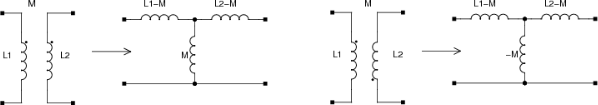
\includegraphics[width=14cm]{./bilder/netzwerkanalyse-kopplung-spulen.png}
\end{center}

\textbf{Vorzeichen der Gegeninduktivität}: 
Fliesst der ``fremde`` (induzierende) Strom bei der \textbf{Markierung hinein}, so hat er dieselbe
Wirkung als wenn er bei der gekoppelten Spule in die \textbf{Markierung
hineinfliessen würde}! 


\subsubsection{Knotenpotentialmethode oder Trennbündelmethode}
\begin{tabular}{ll}
\parbox{6cm}{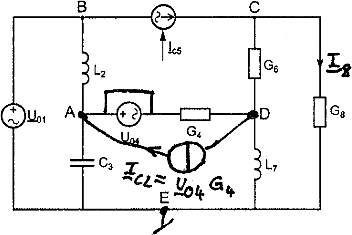
\includegraphics[width=6cm]{./bilder/netzwerkanalyse-knotenpotential.png}
	}
	& \parbox{12cm}{
	Gegeben: $\underline{I}_{C5} = k \underline{I}_8$
	\begin{itemize}
      \item Knoten B hat keine Gleichung, da $E_B = \underline{U}_{01}$
      \item Rechnung nur mit \textit{Admittanzen} (Leitwerten) $\underline{Y}
      = \frac{1}{\underline{Z}} = G + jB$
      \item Schema mit (idealen) \textit{Stromquellen}
    \end{itemize}
$$\begin{bmatrix}
    G_4 + \frac{1}{j \omega L_2} + j \omega C_3 & 0 & -G_4 \\
    0 & G_6 + G_8 - \underbrace{k G_8}_{\underline{I}_{C5}} & -G_6 \\
    -G_4 & -G_6 & \frac{1}{j \omega L_7} + G_4 + G_6   
	\end{bmatrix} \cdot
\begin{bmatrix}
    \underline{E}_A \\ \underline{E}_C \\ \underline{E}_D
    \end{bmatrix} =
\begin{bmatrix}
    \underline{U}_{04} G_4 + \frac{\underline{U}_{01} }{j \omega L_2}\\ 
    0 \\
    -\underline{U}_{04} G_4 \end{bmatrix}$$    
	}
\end{tabular}

$$\textbf{Allgemein: }\left[ \begin{array}{cc}
       \text{Admittanzen $\underline{Y}$} \\
       \text{symmetrisch zur Diagonalen}
%       \text{Diagonale positiv, sonst negativ}
       \end{array}\right] \cdot \left[ \begin{array}{cc}
     \text{Knotenpotentiale $\underline{E}$}
     \end{array}\right] =
\left[ \begin{array}{cc}
     \text{Stromquellen $\underline{J}$} \\
    \text{Hineinfliessen positiv, sonst negativ}
     \end{array}\right]$$

\subsubsection{Aspekte zur Wahl der Methode}
\begin{tabular}{lll}
\multicolumn{3}{l}{\textit{Art der gegebenen Quellen}}\\
&Kreisstrommethode: &Spannungsquellen\\
&Knotenpotentialmethode: &Stromquellen\\
\multicolumn{3}{l}{\textit{Anzahl Gleichungen}}\\ &Kreisstrommethode: &$z-k+1-$ Anzahl idealer Stromquellen\\
&Knotenpotentialmethode: &$k-1-$ Anzahl idealer Spannungsquellen\\
\multicolumn{3}{l}{\textit{Spezialitäten}}\\
&Kreisstrommethode: &Gegeninduktivitäten\\
&Knotenpotentialmethode: &Gesteuerte Stromquellen\\
\multicolumn{3}{l}{\textit{Gesuchte Grössen}}\\
&Kreisstrommethode: &(Sehnen-) Ströme\\
&Knotenpotentialmethode: &(Knoten-) Spannungen
\end{tabular}

\subsection{Stern-Dreieck-Umwandlung}% \formelbuch{18}}
	%\begin{figure}
	  \begin{minipage}[lt]{7.5 cm}
	    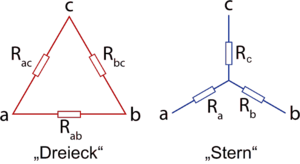
\includegraphics[width=6cm]{./bilder/stern-dreieck.png} 
	  \end{minipage}
	  \begin{minipage}[rt]{9.35 cm} %BASTEL!!
	  \begin{tabular}{ll}
	Umwandlung $\triangle \rightarrow Y$: 
		&$Z_{c} = \dfrac{Z_{ac} Z_{bc}}{Z_{ab}+Z_{bc}+Z_{ac}}$\\
	Umwandlung $Y \rightarrow \triangle$: 
		&$Y_{ac}=\dfrac{Y_{a} Y_{c}}{Y_{a}+Y_{b}+Y_{c}}$\\
	Bei gleichen Widerständen:
	&$R_Y = \frac{R_\triangle}{3}$ \\
	Bei gleichen Kapazitäten:
	&$C_Y = C_\triangle \cdot 3 $ \\
	Bei gleichen Induktivitäten:
	&$L_Y = \frac{L_\triangle}{3}$
	  \end{tabular}
	  \end{minipage}

\subsection{Impedanz-Transformationen}
Werden gebraucht, wenn Bauteile verschiedene Werte haben können. Bspw. wird in
einer Schaltung eine Kapazität oder eine Induktion variiert.\\
%Immer zuerst die einfachere Variante (Serieschaltung: \underline{Z},
%Parallelschaultung: \underline{Y}) darstellen und daraus die andere Ortskurve herleiten. \\
Bei der Umwandlung von \underline{Z} nach \underline{Y} und umgekehrt handelt es sich um die
\textbf{komplexe Kehrwertfunktion}: 
\begin{itemize}
  \item $\underline{Y} = \frac{1}{\underline{Z}} 
  ( arg(\underline{Z}) = -arg(\underline{Y}),  
  |\underline{Y}| = \frac{1}{| \underline{Z} |}) \qquad$
  (Unendlich ferner Punkt wird in den Ursprung abgebildet und umgekehrt)
  \item Verläuft die OK von \underline{Z} oberhalb der Re-Achse, so verläuft die OK von
  \underline{Y} unterhalb der Re-Achse und umgekehrt.
\end{itemize} 
\textbf{Konstruktion} der kreisförmigen Ortskurve:
\begin{enumerate}
  \item Andere Orstkurve (komplexer Kehrwert) als Gerade darstellen. (Dient als Orientierungshilfe
  und zur Überprüfung)
  \item Extremalwerte berechnen und als Punkte $P_1, P_2$ darstellen. 
	($P_1 = \underline{Z}_0 = \lim\limits_{R \rightarrow 0}\underline{Z}, \quad
	  P_2 = \underline{Z}_\infty = \lim\limits_{R \rightarrow \infty}\underline{Z} $)
  \item Mittelsenkrechte von $P_1, P_2$ konstruieren, deren Schnittpunkt mit Re- \textbf{oder}
  Im-Achse den Kreismittelpunkt $M$ ergibt. \\
  Mittels Betrachtung des Anfangswinkels ($\varphi_{Z_0} = - \varphi_{Y_0}$  oder
  $\varphi_{Z_\infty} = - \varphi_{Y_\infty}$) kann die Anfangsrichtung des Kreises in
  der Nähe des Ursprungs bestimmt werden und der ''falsche'' Mittelpunkt ($M_{Re}$ oder $M_{Im}$)
  ausgeschlossen werden.
  \item Ortskurve (Kreis mit Mittelpunkt $M$, schneidet $P_2$ und $P_1$) konstruieren
\end{enumerate}

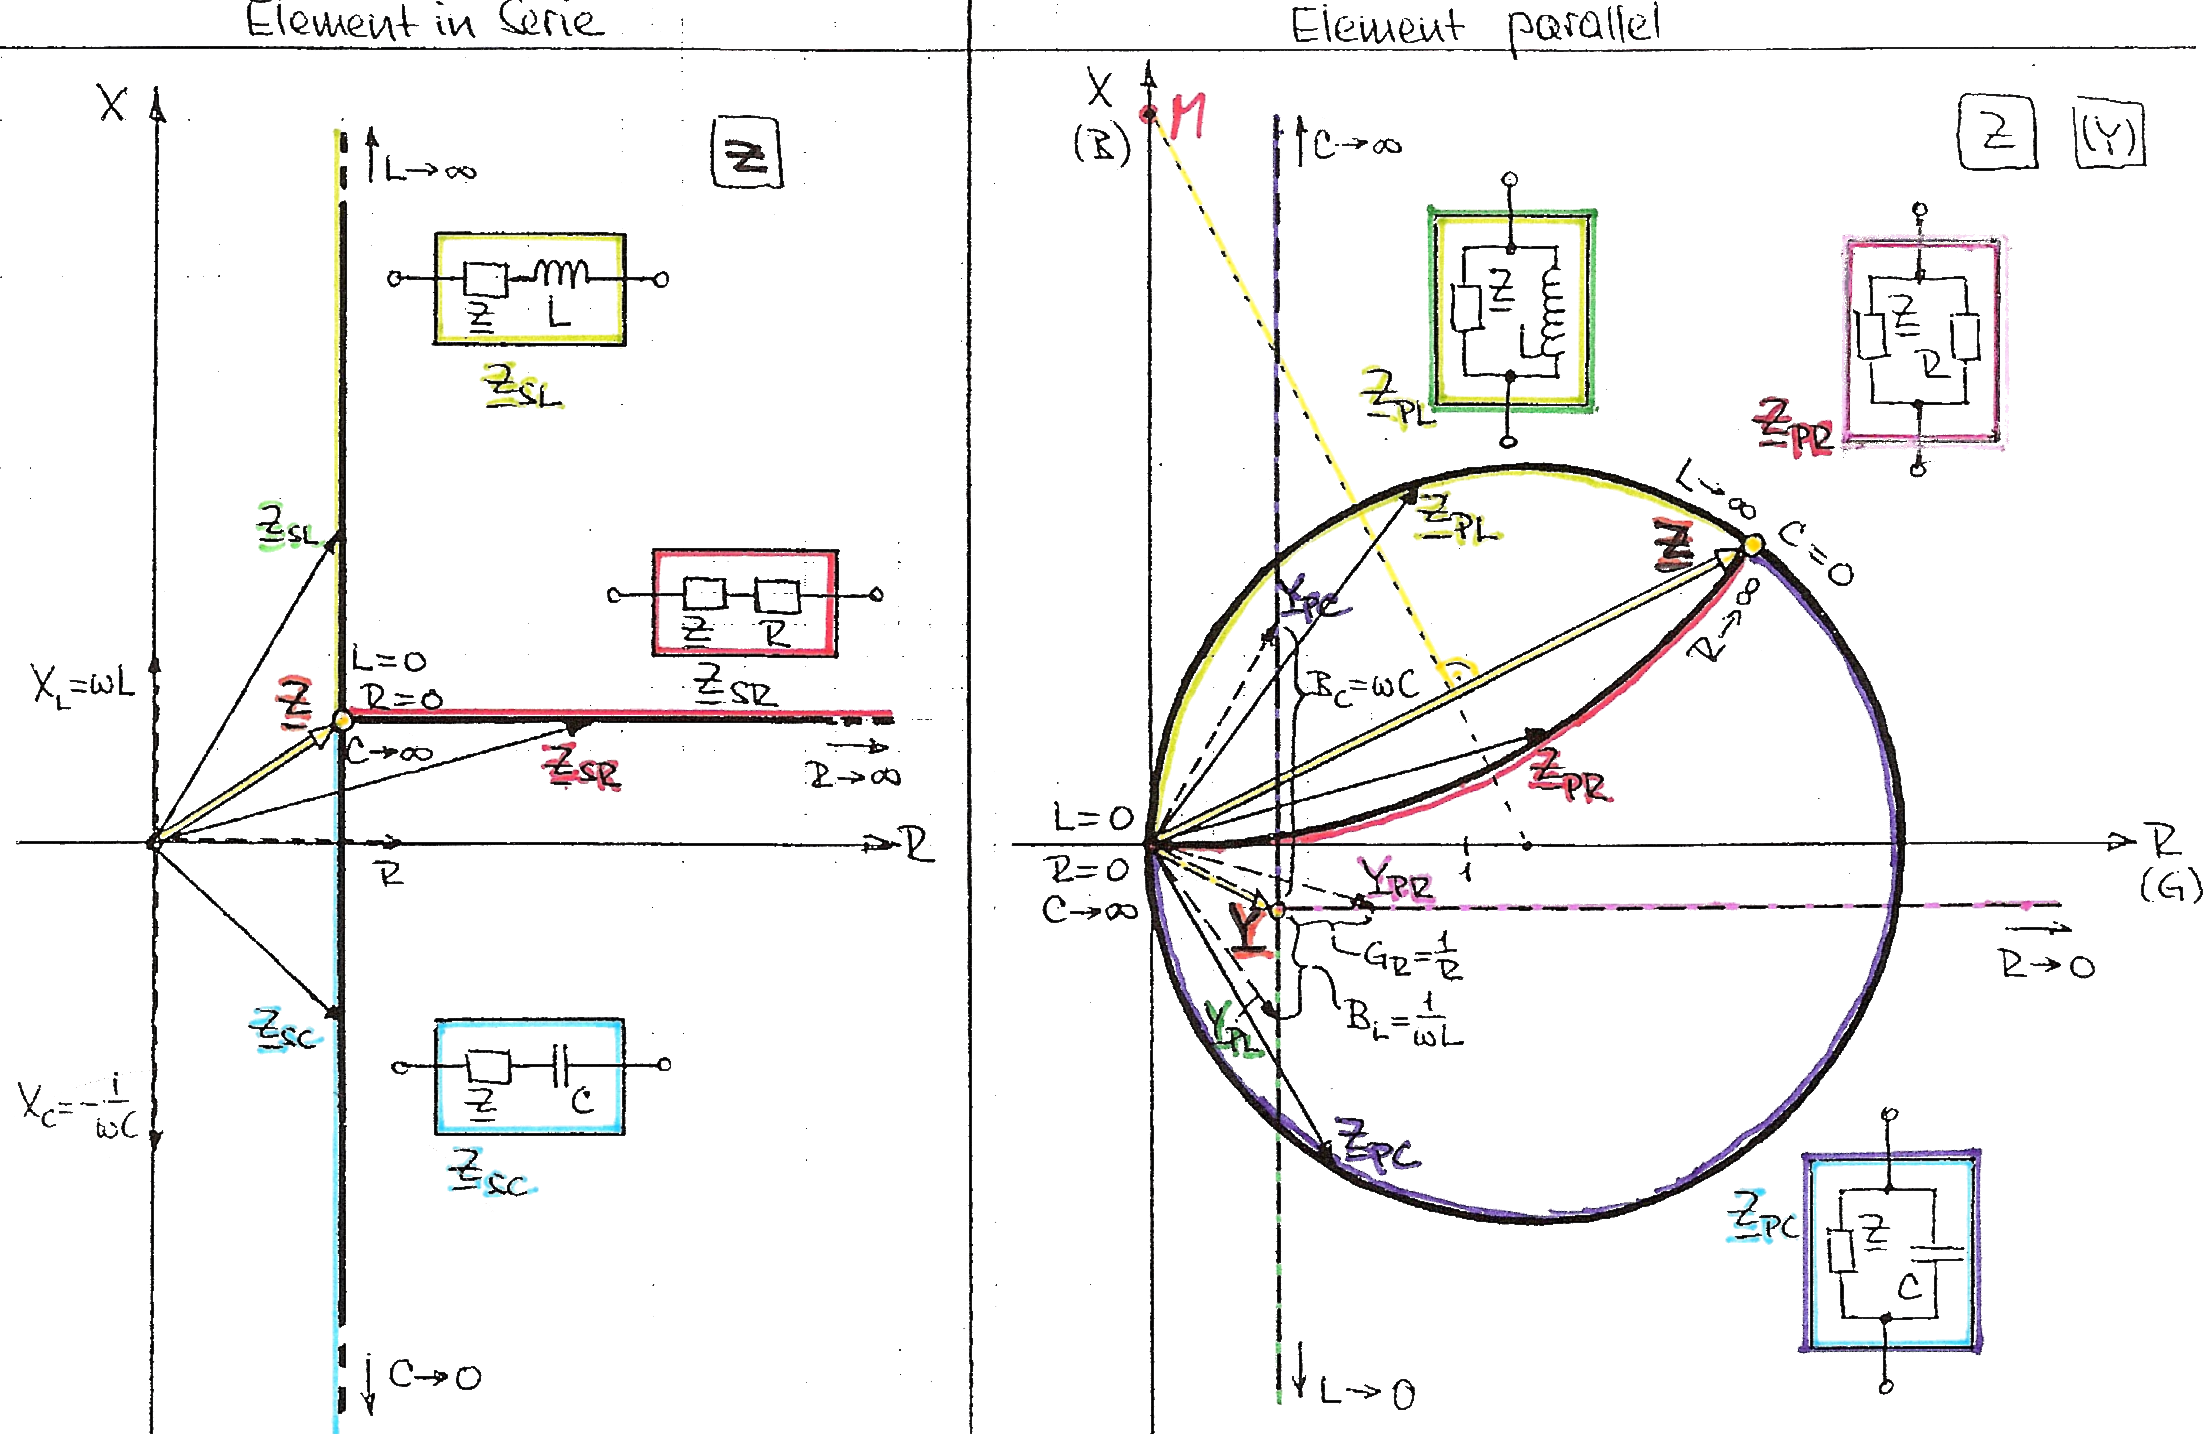
\includegraphics[width=18cm]{./bilder/impedanztrafo.png}